\documentclass[12pt,a4paper]{scrartcl}
\usepackage{scrhack}
\usepackage{scrlayer-scrpage} % Package for header and footer
\usepackage[]{xcolor} % Color package
\usepackage[style=numeric]{biblatex} % Bibliography
\usepackage{xltxtra}
\usepackage{fontspec} % Font package
\usepackage[T1]{fontenc}
\usepackage{xunicode}
\usepackage{inconsolata} % Add inconsolata monospaced font
\usepackage[a4paper]{geometry}
\usepackage{subfig}
\usepackage{graphicx}
\usepackage{palatino}
\usepackage{float} % Float placement
\usepackage[english, french]{babel} % Languages
\usepackage{csquotes}
\usepackage[hidelinks]{hyperref} % Add clickable links
\usepackage[acronym, section]{glossaries}
\usepackage[noabbrev]{cleveref} % Better references
\usepackage{listings} % Code listings
\usepackage{lipsum} 
\usepackage{dirtytalk}

% Configure paragraph look
\setlength{\parskip}{1em}
\setlength{\parindent}{0em}

% Configure name for listings in creferences
\crefname{lstlisting}{listing}{listings}
\Crefname{lstlisting}{Listing}{Listings}

% Configure listings
\lstset{ 
	keywordstyle=\color{mygreen},
	stringstyle=\color{orange},
	breaklines=true,
	numbers=left,
	basicstyle=\ttfamily\footnotesize,
	captionpos = b
}

\setmonofont{inconsolata}

\begin{document}
\begin{titlepage}
	\centering
	
\includegraphics[width=0.66\textwidth]{img/title_logo.png}\par\vspace{1cm}
	{\scshape\LARGE Polytech Montpellier\par}
	\vspace{1cm}
	{\scshape\Large Functional Programming Project\par}
	\vspace{1.5cm}
	{\huge\bfseries SGit\par}
	\vspace{2cm}
	{\Large\itshape Yannick Mayeur\par}
	\vfill
	supervised by\par
	Arnaud \textsc{Castelltort}\par

	\vfill

% Bottom of the page
	{\large \today\par}
\end{titlepage}

\tableofcontents
\break


\section{Introduction}

Git is distributed version-control system for tracking changes in source code.
Git's architecture is very much based on the concept of immutable
data structure.

Scala is a multi-paradigm language providing support for functional
programming. Functional programming is a programming paradigm that bases a lot
of its strength on immutable data structures and on the manipulation  of this
data with pure functions.

Trying to do an implementation of a Git-like tool with Scala thus seems like a
perfect match. In this document we will see how the tool can be installed and
used, then we will tackle the architecture of the application with its pros and
cons and finally we will do a conclusion of the project and try to analyze
elements that went right but also elements that went wrong.

\section{Instructions}

\subsection{Requirements}

In order to build and run the project it is required to have:

\begin{itemize}
		\item Scala version 2.13.0
		\item sbt version 1.3.2
		\item Java 8 JDK
\end{itemize}

\subsection{Installation guide}
The source code for the application is is hosted on GitHub at the following
URL: \url{https://github.com/yannick-mayeur/sgit}.

To build the project from the sources execute the following bash instructions:

\begin{lstlisting}
$ git clone https://github.com/yannick-mayeur/sgit.git sgit-yannickm
$ cd sgit-yannickm
$ sbt assembly
\end{lstlisting}

The binary is generated into \lstinline{target/scala-2.13}. You can add the
path to this folder to your \lstinline{PATH} variable to be able to launch sgit
commands from anywhere on your system.

To get an overview of available commands execute the following command:

\begin{lstlisting}
$ sgit --help
\end{lstlisting}

\section{Architecture of the application}
Git is implemented in the C programming language and in order to maximize
performance it relies heavily on reading and writing to files and has almost no
internal data structure. With a functional programming language like Scala, I/O
should be avoided as much as possible to take advantage of the power of the
paradigm. And having data structures makes it easier for a human to reason
about the code because they introduce abstraction.
\begin{figure}[h]
	\centering
	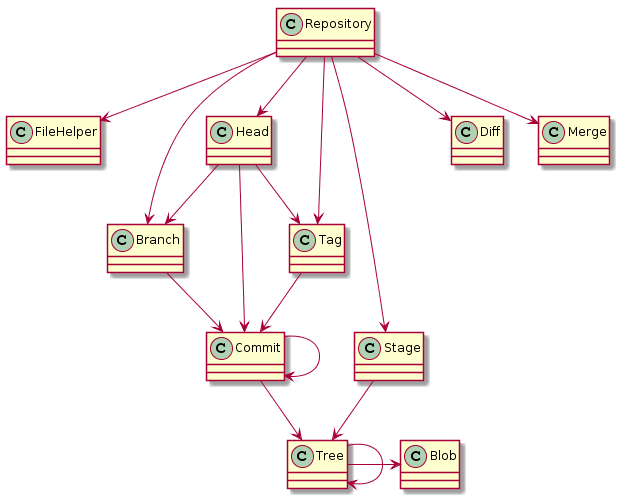
\includegraphics[width=0.8\textwidth]{img/diagram.png}
	\caption{Architecture of the application}
	\label{fig:architecture}
\end{figure}

To reduce everything related to State and I/O to a minimum all I/O functions
required in the code are grouped into the \lstinline{FileHelper} class. This
class is injected in the \lstinline{Repository} Singleton Object and then in the
\lstinline{Repository} object. The \lstinline{Repository} object then becomes
the cornerstone of the application, because it will pass as an argument the
function that the other objects require to correctly compute the result of
their calculations. These passed functions transparently enable the objects to
do I/O without knowing about it, and thus reduces coupling with the file based data
structure. This architecture can be seen on \Cref{fig:architecture}.


\subsection{Pros}
This architecture comes with some advantages. The biggest one is in my opinion
the ability to reason about the lower levels of the program without
having to think about I/O or the file system, because everything is handled by
the  Repository.

Another big one is that it makes testing the program very easy. Indeed most
functions only depend on their parameters and thus produce a predictable
result, this is called referential transparency. In the different tests all I
had to do was to mock the functions given as parameters to easily test isolated
bits of the code.

\begin{lstlisting}[caption = Scala code example, label = lst:code1]
Diff
  .getDiffBetweenTrees(t1, t2)
  .map(_.formatChanges(printDiff))
  .mkString("\n")
\end{lstlisting}

And last but not least having a lot of different small data structures greatly
improves the readability of code. The abstraction introduced by this makes some
parts of code almost as readable as a good book. On \cref{lst:code1} this is
very obvious, we get the difference between two trees, we then format the
changes to print the difference between them, and finally we separate each
change by a line break to make it a printable string.

\subsection{Cons}
The architecture is far from being perfect and comes with some drawbacks. The
biggest one in my opinion being that the objects at the higher levels of the
architecture often take a lot of arguments, they pass down to the other
objects. This sometimes makes it hard to read the signature of some functions.

The other major one is that a lot of the logic starts in the
\lstinline{Repository} and thus makes it a very long and hard to read class.

\section{Testing strategy}

\subsection{The end strategy}
As I already said one of the strength of programming in a functional manner is
that for a set of parameters a function returns a predictable result.

Thus doing unit tests is ideal, because we check that each function does its
job correctly.

To verify that the different blocks work good together I also did integration
tests. These tests are done by testing the \lstinline{Repository} object,
because this object relies on all other objects to correctly produce the result
for its functions. To test the \lstinline{Repository} a mock of the
\lstinline{FileHelper} was done with the help of the Mockito Scala library.

\subsection{A struggling start}
The architecture of application evolved a lot during the project to find a way
to get rid as much I/O and State as possible. The early version of the project
relied on a lot on I/O for the tests, which I did not like at all.

This problem is what finally made me decide to do a huge refactoring of the
code that would allow to easily do test-driven development, and boost my
productivity.

\section{Post Mortem}

\subsection{What went right}
For this project I set up a big development environment. I used Travis to do
continuous integration. GitHub to host the code and handle my pull requests
that were only mergeable once Travis said the code was good, and to track the
issues the project. Organizing the project in a "professional" way takes off a lot
of weight of the project, because it helps to do quality code and to track
the project as a whole.

Even if it is a solo project teamwork was central to the project. I discussed
architectures and algorithms a lot with Thomas Falcone, Lucas Gonçalves and
Paul Arnaud. I think that this teamwork greatly improved the quality of our
final projects because it allowed us to always have a critical opinion on our
ideas.

\subsection{What went wrong}
No project every happened without some things going wrong. This project is no
exception to the rule.

The biggest problem I had was that after I understood the project and that my
development environment was set up, I dove almost blindly into coding, thinking
that some quick refactoring could clean up the code in later stages. 

A few hundred lines of code later I had myself a beautiful Big Ball of Mud.

\say{A Big Ball of Mud
is a haphazardly structured, sprawling, sloppy, duct-tape-and-baling-wire,
spaghetti-code jungle}. Quote by Brian Foote and Joseph Yoder.

Thankfully I could identify the problem in time but because of the bad start
architecture, tests were very hard to write, which made refactoring very hard
because there was no easy way of seeing if regressions happened.

Once the architecture was refactored and good tests were written it was a
thousand times easier to make easy changes and write new functionalities.

Today with dark circles under my eyes I can say that I regret my eagerness to
code fast, and that next time I will think twice before jumping into
development.

\end{document}
